\documentclass[border=1pt]{standalone}
\usepackage[dvipsnames]{xcolor}
\usepackage{tikz}                       % Graphen und kommutative Diagramme
\usetikzlibrary{patterns}               % Um schraffierte Formen in der tikzpicture-Umgebung zu zeichnen.

\begin{document}

\newcommand{\ul}{\underline}
\newcommand{\radmult}
{
    \ensuremath{
	\tikz[baseline={([yshift=-1pt]current bounding box.center)}, x=5pt, y=2.5pt, every node/.style={shape=circle, fill=black, inner sep=.8pt}]{
	    \draw[line width=0.9pt] (5, 0) -- (3, 0);
	    \draw[line width=0.9pt] (2, 0) -- (0, 0);
	    \filldraw (3, 0) circle (1pt);
	    \filldraw (2, 0) circle (1pt);
	}
    }
}

\newcommand{\equals}
{
    \ensuremath{
	\tikz[baseline={([yshift=2pt]current bounding box.center)}, x=5pt, y=2.5pt]{
	    \node (0, 0) {$=$};
	}
    }
}
\begin{minipage}{.55\textwidth}
\centering
\resizebox{!}{3.5cm}{
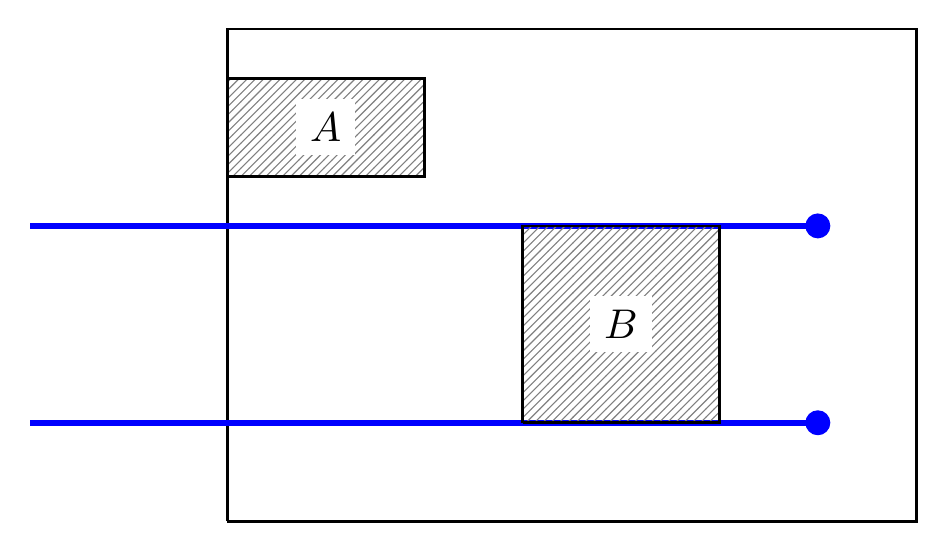
\begin{tikzpicture}[x=1.25cm, y=1.25cm, line width=1pt]
    % draw outer lines
    \draw (1, 0) -- (8, 0) -- (8, 5) -- (1, 5) -- (1, 0);
    
    % draw slits
    
    \draw[color=blue, line width=2pt] (-1, 1) -- (7, 1);
    \filldraw[color = blue, fill = blue] (7, 1) circle (4pt);
   
    \draw[color=blue, line width=2pt] (-1, 3) -- (7, 3);
    \filldraw[color = blue, fill = blue] (7, 3) circle (4pt);

    % draw shaded slit box
    \filldraw[pattern=north east lines, pattern color=black!50] (1, 3.5) -- (3, 3.5) -- (3, 4.5) -- (1, 4.5) -- (1, 3.5);
    \filldraw[pattern=north east lines, pattern color=black!50] (4, 1) -- (6, 1) -- (6, 3) -- (4, 3) -- (4, 1);
     
    % draw symbols
    
    \node[scale = 1.5, fill = white] at (2, 4) {$A$};
    \node[scale = 1.5, fill = white] at (5, 2) {$B$};
\end{tikzpicture}
}
\end{minipage}

\begin{minipage}{.55\textwidth}
\centering
\resizebox{!}{3.5cm}{
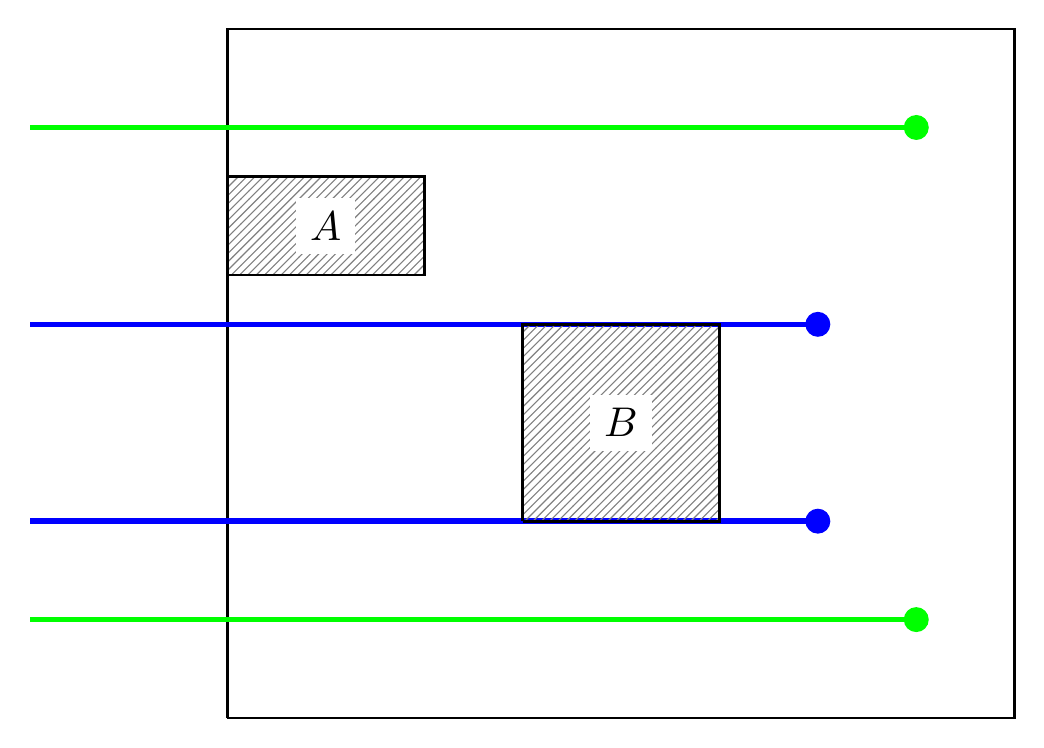
\begin{tikzpicture}[x=1.25cm, y=1.25cm, line width=1pt]
    % draw outer lines
    \draw (1, 0) -- (9, 0) -- (9, 7) -- (1, 7) -- (1, 0);
    
    % draw slits
    
    \draw[color=green, line width=2pt] (-1, 1) -- (8, 1);
    \filldraw[color = green, fill = green] (8, 1) circle (4pt);
    
    \draw[color=blue, line width=2pt] (-1, 2) -- (7, 2);
    \filldraw[color = blue, fill = blue] (7, 2) circle (4pt);
    
    \draw[color=blue, line width=2pt] (-1, 4) -- (7, 4);
    \filldraw[color = blue, fill = blue] (7, 4) circle (4pt);

    \draw[color=green, line width=2pt] (-1, 6) -- (8, 6);
    \filldraw[color=green, fill = green] (8, 6) circle (4pt);
    % draw shaded slit box
    \filldraw[pattern=north east lines, pattern color=black!50] (1, 4.5) -- (3, 4.5) -- (3, 5.5) -- (1, 5.5) -- (1, 4.5);
    \filldraw[pattern=north east lines, pattern color=black!50] (4, 2) -- (6, 2) -- (6, 4) -- (4, 4) -- (4, 2);
     
    % draw symbols
    
    \node[scale = 1.5, fill = white] at (2, 5) {$A$};
    \node[scale = 1.5, fill = white] at (5, 3) {$B$};
\end{tikzpicture}}
\end{minipage}

\end{document}